\task{ Найдите сопротивление между точками $A$ и $B$ в цепи,
  изображённой на рисунке. Сопротивление каждого из ребёр составляет
  $R$. Цепь бесконечна в обе стороны.}
\begin{center}
  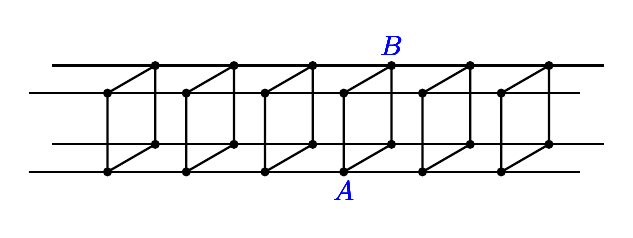
\begin{tikzpicture}
    \foreach \x in {0,1,...,5}
    {
      \draw[thick] (\x,0) -- (\x,1) -- ++(30:0.7cm) -- ++(-90:1cm) --
      cycle;
      \draw[fill=black] (\x,0) circle (0.05cm) (\x,1) circle (0.05cm) 
      ++(30:0.7cm) circle(0.05cm)  ++(-90:1cm) circle (0.05cm);
      \draw[thick] (-1,0) -- (6,0);
      \draw[thick,yshift=0.35cm,xshift=0.3cm] (-1,0) -- (6,0);
      \draw[thick] (-1,1) -- (6,1);
      \draw[thick,yshift=0.35cm,xshift=0.3cm] (-1,1) -- (6,1);
      \draw (3,0) node[below,blue] {$A$};
      \draw (3,1) ++ (30:0.7cm) node[above,blue] {$B$};
    }
    
  \end{tikzpicture}
\end{center}
% Белорусские олимпиады, 1991, №3
